\section{Experiments}
\label{sec:experiments}
In our experiments, we evaluate \phil both on benchmark heuristic learning datasets \cite{bhardwaj2017learning} (Section \ref{sec:experiments-grids}) as well on a diverse set of graph datasets (Section \ref{sec:experiments-diversity}). Finally, we show that \phil can be applied to efficient planning in the context of drone flight (Section \ref{sec:experiments-drone}). Our main goal is to assess how \phil compares to baseline methods in terms of necessary expansions before the goal node is reached.


\subsection{Heuristic search in grids}
\label{sec:experiments-grids}

\begin{wrapfigure}[13]{r}{0.3\textwidth}
  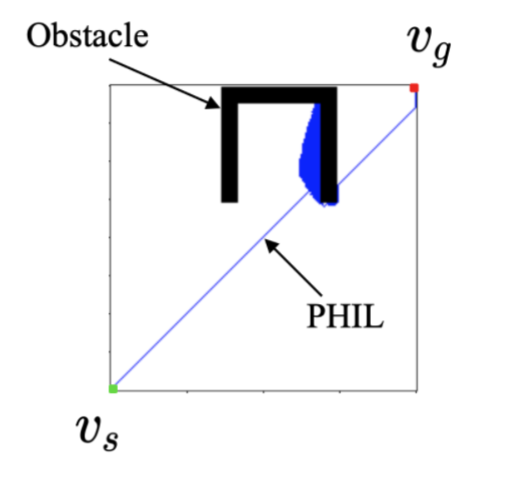
\includegraphics[width=\linewidth]{figures/local_minima.png}
    \caption{Example of \phil escaping local search minima.}
  \label{fig:local-min}
\end{wrapfigure}


In Section \ref{sec:experiments-grids}, we evaluate \phil on $8$, $200 \times 200$ 8-connected grid graph-based datasets by Bhardwaj \etal \cite{bhardwaj2017learning}. These datasets present challenging obstacle configurations for naive greedy planning heuristics, especially when $v_s$ is in the bottom-left of the grid, and $v_g$ in the top-right. Each dataset contains 200 training graphs, 70 validation graphs, and 100 test graphs. Example graphs from each dataset can be found in Table \ref{tab:table-1}.


We train \phil with a hyperparameter configuration of $T = 128$,  $t_{\tau} = 32$, $\beta_{0} = 0.7$, $n = 8$, and using rolled-in $z_t$ states as initial states for training. We use a 3-layer $\textsc{MLP}$ of width 128 with \textit{LeakyReLU} activations, followed by a DeeperGCN \cite{li2020deepergcn} graph convolution with \textit{softmax} aggregation. Our memory’s embedding dimensionality is $64$. The node features are 2D grid coordinates. Note that although using positional representations \cite{you2019position} might be useful for this search problem, it is not scalable as the graph size increases.

\begin{table*}[!htb]
\centering
\caption{The number of expanded graph nodes of \phil with respect to \sail. We can observe that out of all baselines, \sail performs best. \phil outperforms \sail by $58.5 \%$ on average over all datasets, with a maximal search effort reduction of $82.3 \%$ in the \textit{Gaps+Forest} dataset.}
\label{tab:table-1}
\resizebox{\columnwidth}{!}{%

\begin{tabular}{ccccccccccccccc} \toprule
 \textbf{Dataset} & \multicolumn{3}{c}{\textbf{Graph Examples}} & \textbf{\sail} & \textbf{SL} & \textbf{CEM} & \textbf{QL} & \textbf{$h_{euc}$} & \textbf{$h_{man}$} & \textbf{A*} & \textbf{MHA*} & \textbf{BFWS} & \textbf{Neural A*} & \textbf{\phil} \\ \midrule

Alternating gaps    & \frame{
\includegraphics[width=0.6cm, height=0.6cm]{figures/alt_1.png}} &  \frame{
\includegraphics[width=0.6cm, height=0.6cm]{figures/alt_2.png}}  &  \frame{
\includegraphics[width=0.6cm, height=0.6cm]{figures/alt_3.png}}   &0.039	&0.432& 0.042	& 1.000 & 1.000	&1.000	&1.000 & 1.000 & 0.34 &0.546 &\textbf{0.024}\\ 
Single Bugtrap       & \frame{
\includegraphics[width=0.6cm, height=0.6cm]{figures/sb1.png}} & \frame{
\includegraphics[width=0.6cm, height=0.6cm]{figures/sb2.png}}  & \frame{
\includegraphics[width=0.6cm, height=0.6cm]{figures/sb3.png}} 	& 0.158	& 0.214	& 0.057	& 1.000	&0.184	&0.192	&1.000	&0.286 & 0.099 &0.394 & 
\textbf{0.077} \\ 
Shifting gaps       & \frame{
\includegraphics[width=0.6cm, height=0.6cm]{figures/sg1.png}}  & \frame{
\includegraphics[width=0.6cm, height=0.6cm]{figures/sg2.png}}  & \frame{
\includegraphics[width=0.6cm, height=0.6cm]{figures/sg3.png}}  &0.104	&0.464	&1.000	&1.000	&0.506	&0.589	&1.000	&0.804 & 0.206 &0.563 &\textbf{0.027} \\
Forest              & \frame{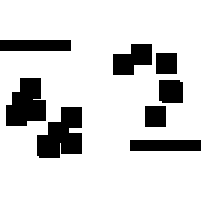
\includegraphics[width=0.6cm, height=0.6cm]{figures/f_1.png}}  & \frame{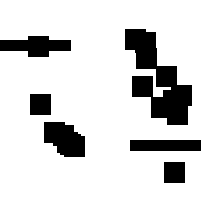
\includegraphics[width=0.6cm, height=0.6cm]{figures/f2.png}}  &  \frame{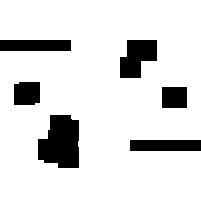
\includegraphics[width=0.6cm, height=0.6cm]{figures/f3.png}}   & 0.036 &0.043	&0.048	&0.121	&0.041	&0.043	&1.000	&0.075 & 0.039  &0.399 & \textbf{0.027}\\
Bugtrap+Forest      & \frame{
\includegraphics[width=0.6cm, height=0.6cm]{figures/bf_1.png}}  & \frame{
\includegraphics[width=0.6cm, height=0.6cm]{figures/bf_2.png}}  &  \frame{
\includegraphics[width=0.6cm, height=0.6cm]{figures/bf_3.png}}  	&0.147	&0.384	&0.182	&1.000	&0.410	&0.337	&1.000	&3.177 & 0.149 &0.651 &\textbf{0.135} \\
Gaps+Forest         &\frame{ 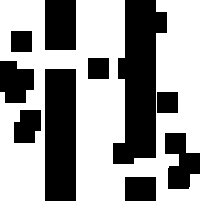
\includegraphics[width=0.6cm, height=0.6cm]{figures/gf1.png}}  & \frame{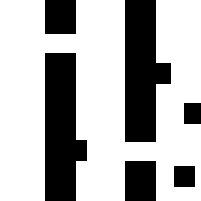
\includegraphics[width=0.6cm, height=0.6cm]{figures/gf2.png}}  & \frame{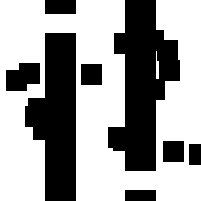
\includegraphics[width=0.6cm, height=0.6cm]{figures/gf3.png}}    	&0.221	&1.000	&1.000	&1.000	&1.000	&1.000	&1.000	&1.000 & 0.401 & 0.580 &\textbf{0.039} \\
Mazes               & \frame{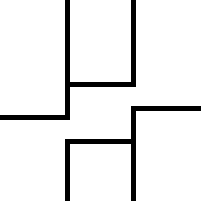
\includegraphics[width=0.6cm, height=0.6cm]{figures/m1.png}}  & \frame{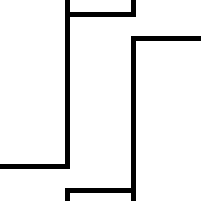
\includegraphics[width=0.6cm, height=0.6cm]{figures/m2.png}}  & \frame{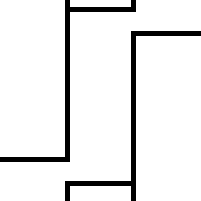
\includegraphics[width=0.6cm, height=0.6cm]{figures/m3.png}} 	&0.103	&0.238	&0.479	&0.399	&0.185	&0.171	&1.000	&0.279 & 0.095 &1.000 &\textbf{0.069}\\
Multiple Bugtraps   & \frame{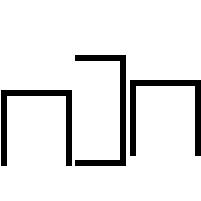
\includegraphics[width=0.6cm, height=0.6cm]{figures/mb1.png}}  & \frame{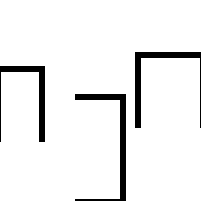
\includegraphics[width=0.6cm, height=0.6cm]{figures/mb2.png}}  & \frame{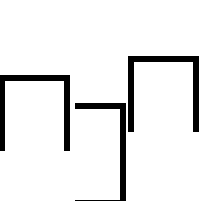
\includegraphics[width=0.6cm, height=0.6cm]{figures/mb3.png}} 	&0.479	&0.480	&1.000	&0.835	&0.648	&0.617	&1.000	&0.876 &0.169 &0.331 & \textbf{0.136}  \\ \bottomrule

% Alternating gaps    & \frame{
\includegraphics[width=0.6cm, height=0.6cm]{figures/alt_1.png}} &  \frame{
\includegraphics[width=0.6cm, height=0.6cm]{figures/alt_2.png}}  &  \frame{
\includegraphics[width=0.6cm, height=0.6cm]{figures/alt_3.png}}   &1.000	&11.077	&1.077	&25.641	&25.641	&25.641	&25.641	&25.641 & 8.718 & &\textbf{0.615}\\ 
% Single Bugtrap       & \frame{
\includegraphics[width=0.6cm, height=0.6cm]{figures/sb1.png}} & \frame{
\includegraphics[width=0.6cm, height=0.6cm]{figures/sb2.png}}  & \frame{
\includegraphics[width=0.6cm, height=0.6cm]{figures/sb3.png}} 	&1.000	&1.354	&\textbf{0.361}	&6.329	&1.165	&1.215	&6.329	&1.772 & 0.625 & & 0.544 \\ 
% Shifting gaps       & \frame{
\includegraphics[width=0.6cm, height=0.6cm]{figures/sg1.png}}  & \frame{
\includegraphics[width=0.6cm, height=0.6cm]{figures/sg2.png}}  & \frame{
\includegraphics[width=0.6cm, height=0.6cm]{figures/sg3.png}}      &1.000	&4.462	&9.615	&9.615	&4.865	&5.663	&9.615	&7.731 & 1.982 & &\textbf{0.260} \\
% Forest              & \frame{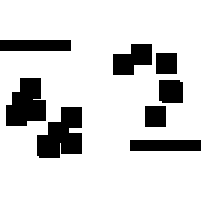
\includegraphics[width=0.6cm, height=0.6cm]{figures/f_1.png}}  & \frame{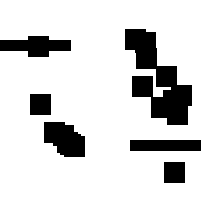
\includegraphics[width=0.6cm, height=0.6cm]{figures/f2.png}}  &  \frame{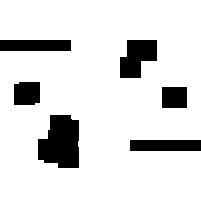
\includegraphics[width=0.6cm, height=0.6cm]{figures/f3.png}}             &1.000	&1.194	&1.333	&3.361	&1.139	&1.194	&27.778	&2.083 & 1.078 & & \textbf{0.778}\\
% Bugtrap+Forest      & \frame{
\includegraphics[width=0.6cm, height=0.6cm]{figures/bf_1.png}}  & \frame{
\includegraphics[width=0.6cm, height=0.6cm]{figures/bf_2.png}}  &  \frame{
\includegraphics[width=0.6cm, height=0.6cm]{figures/bf_3.png}}  	&1.000	&2.612	&1.238	&6.803	&2.789	&2.293	&6.803	&3.177 & 1.011 & &\textbf{0.810} \\
% Gaps+Forest         &\frame{ 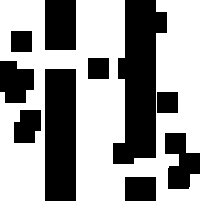
\includegraphics[width=0.6cm, height=0.6cm]{figures/gf1.png}}  & \frame{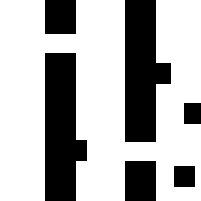
\includegraphics[width=0.6cm, height=0.6cm]{figures/gf2.png}}  & \frame{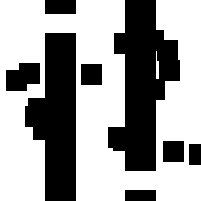
\includegraphics[width=0.6cm, height=0.6cm]{figures/gf3.png}}    	&1.000	&4.525	&4.525	&4.525	&4.525	&4.525	&4.525	&4.525 & 1.813 & &\textbf{0.213} \\
% Mazes               & \frame{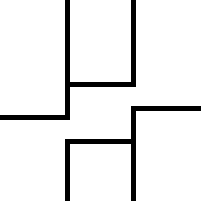
\includegraphics[width=0.6cm, height=0.6cm]{figures/m1.png}}  & \frame{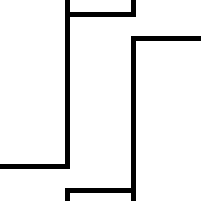
\includegraphics[width=0.6cm, height=0.6cm]{figures/m2.png}}  & \frame{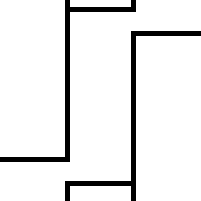
\includegraphics[width=0.6cm, height=0.6cm]{figures/m3.png}} 	&1.000	&2.311	&4.650	&3.874	&1.796	&1.660	&9.709	&2.709 & 0.921 & &\textbf{0.495}\\
% Multiple Bugtraps   & \frame{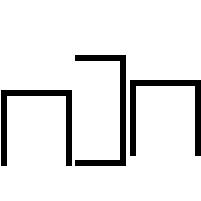
\includegraphics[width=0.6cm, height=0.6cm]{figures/mb1.png}}  & \frame{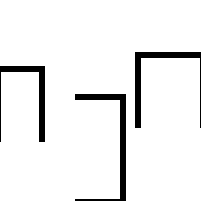
\includegraphics[width=0.6cm, height=0.6cm]{figures/mb2.png}}  & \frame{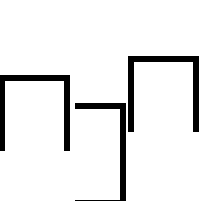
\includegraphics[width=0.6cm, height=0.6cm]{figures/mb3.png}} 	&1.000	&1.002	&2.088	&1.743	&1.353	&1.288	&2.088	&1.829 &0.353 & & \textbf{0.382}  \\ \bottomrule
\end{tabular}
}
\end{table*}

%\jure{Could we add squares/boxes around Graph Examples (as in Fig 4). I think then it will be much clearer that these are same things as in Fig 4).}
%\jure{Caption: Rather than discussing the baselines let's discuss performance and point out interesting observations. For example: ``Out of all baselines \sail performs best, while PHIL performs X\% better than \sail on average.'' Let's say something like this.} \update{boxes and quantified observations added}

\textbf{Discussion.} As we can see in Table \ref{tab:table-1}, \phil outperforms the best baseline (\textit{\sail}) on all datasets, with an average reduction of explored nodes before $v_g$ is found of $58.5 \%$.
%Even with \textit{CEM} performing better than \phil on \textit{Single Bugtrap}, \phil reduces the necessary search effort compared with the best baseline on each dataset by \michal{$40.8 \%$} on average.
Qualitatively, observing Figure \ref{fig:sail-comparison}, we can attribute these results to \phil's ability to \textbf{reduce the redundancy in explored nodes} during a search. Further, \phil is also \textbf{capable of escaping local minima}, which is illustrated in Figure \ref{fig:local-min}. However, note that we occasionally observe failure cases in practice, where \phil gets stuck in a bug trap-like structure.

\xhdr{Runtime \& convergence speed} \phil converges in up to $N = 36$ iterations, with $m = 1, t_\tau = 32$ (i.e., after observing less than $N * t_\tau * max(|\VS_{new}|) \approx 9,216$ shortest path distances, where we take $max(|\VS_{new}|) = 8$ as the maximal size of $\VS_{new}$). According to figures reported in \cite{bhardwaj2017learning}, this is approximately $5\times$ less data than it takes for \sail to converge.
%Although neither the \sail or \phil code-bases were optimized for runtime speed, we found that our implementation of \phil runs about $7 \times$ faster than the publicly available implementation of \sail on the \textit{Gaps+Forest} dataset.


%\jure{Same here, can we quantify performance: PHIL explores X\% less nodes on average than the second best method, Sail} \update{Should be better quantified \& more optimistic}
% \setlength{\framerule}{1pt}%

\begin{figure*}[h!]
    \centering
    \begin{adjustbox}{minipage=\linewidth,scale=0.9}

    \begin{subfigure}[t]{0.45\textwidth}
         \raisebox{-\height}{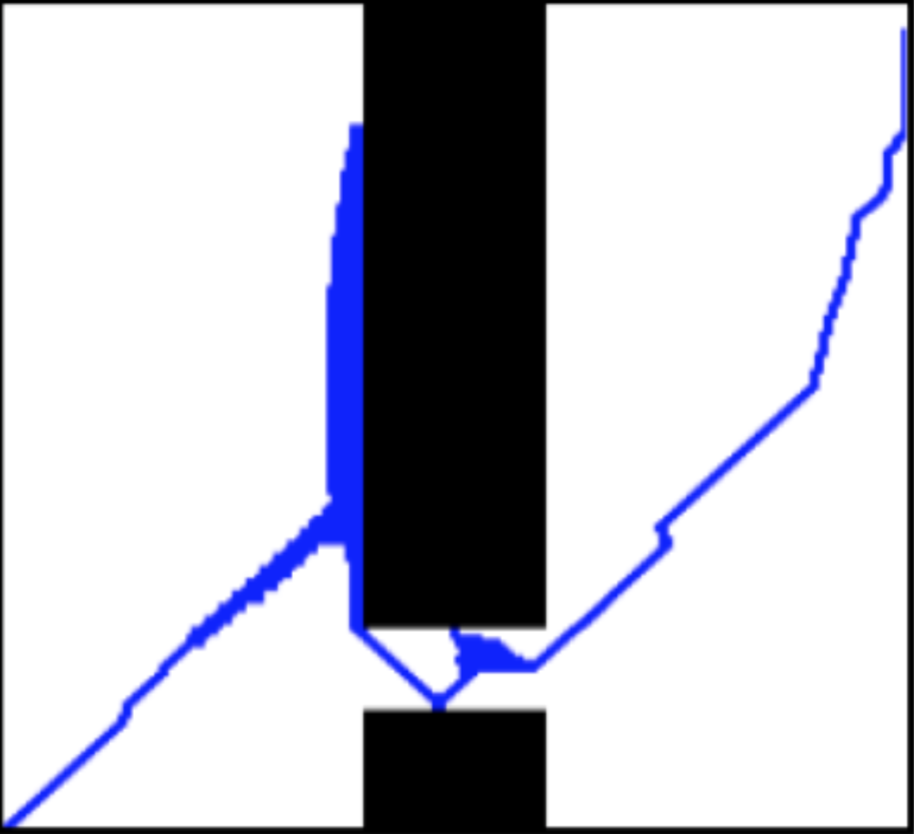
\includegraphics[width=0.49\textwidth,height=0.49\textwidth]{figures/c1_sail.png}}
         \raisebox{-\height}{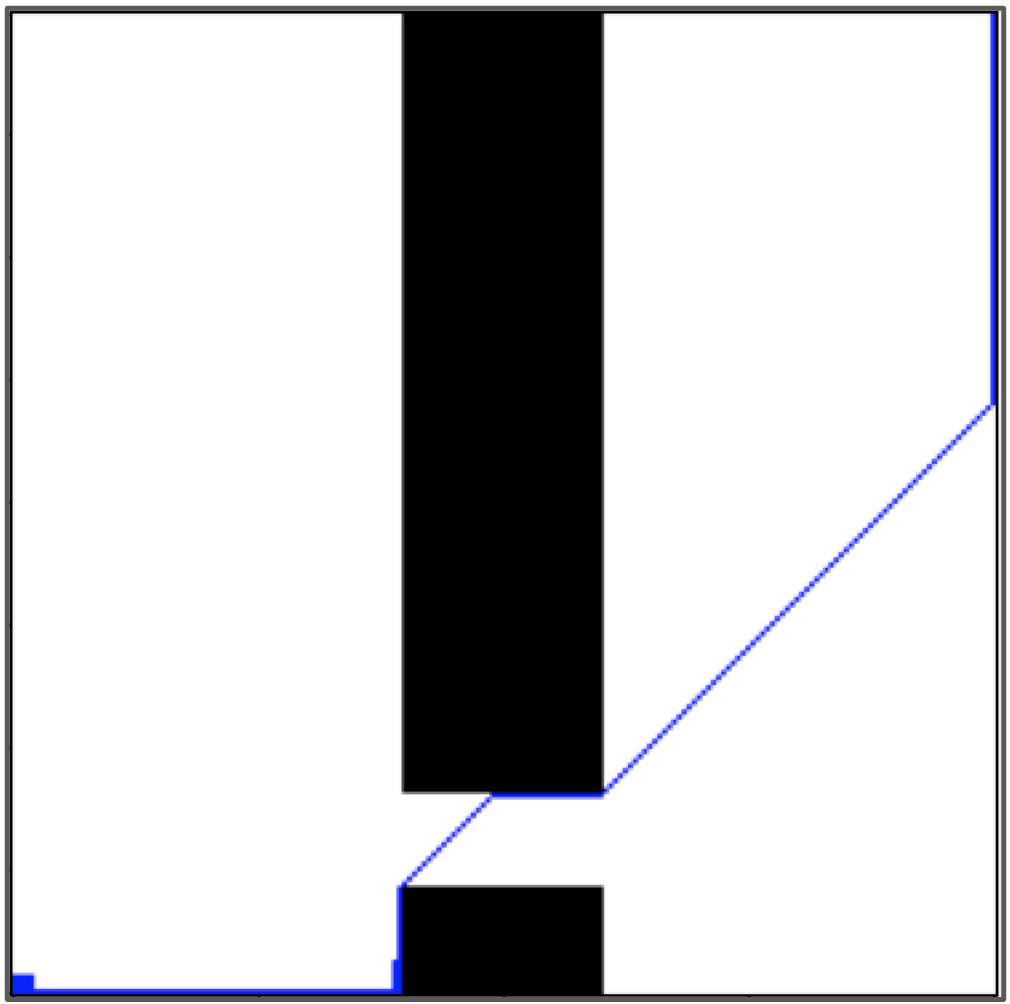
\includegraphics[width=0.49\textwidth,height=0.49\textwidth]{figures/c1.png}}%
         \label{fig:one-a}
    \caption{Shifting gaps (\sail left, \phil right)}
    \end{subfigure}
    \hfill
    \begin{subfigure}[t]{0.45\textwidth}
         \raisebox{-\height}{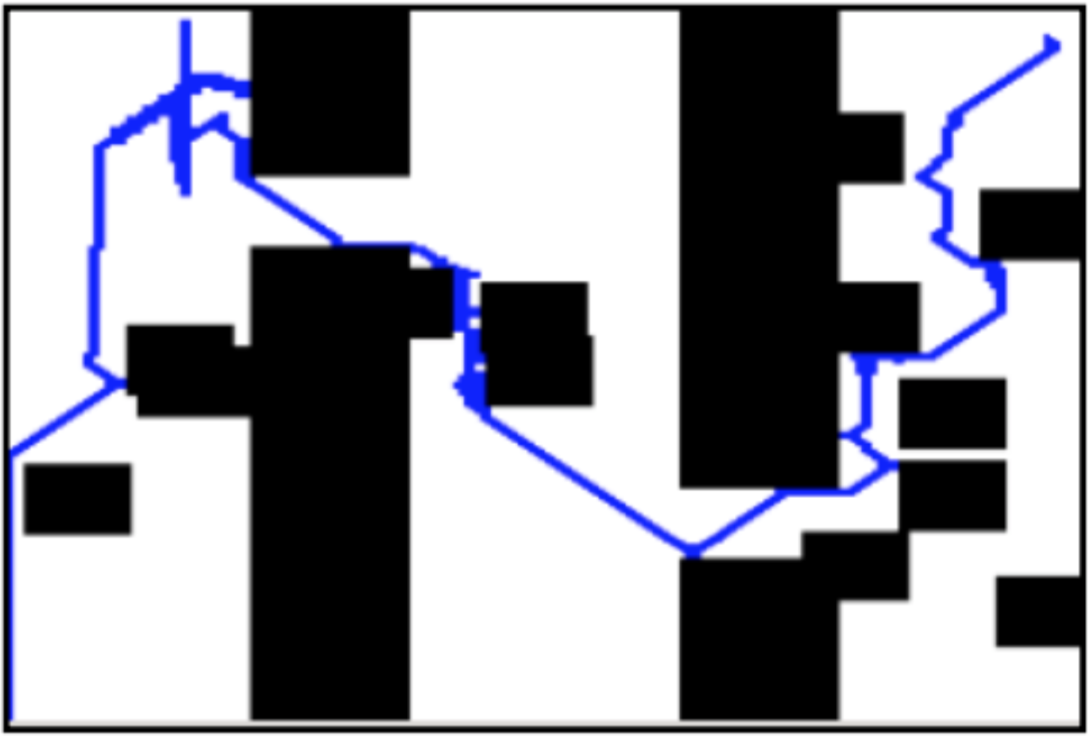
\includegraphics[width=0.49\textwidth,height=0.49\textwidth]{figures/c2_sail.png}}
         \raisebox{-\height}{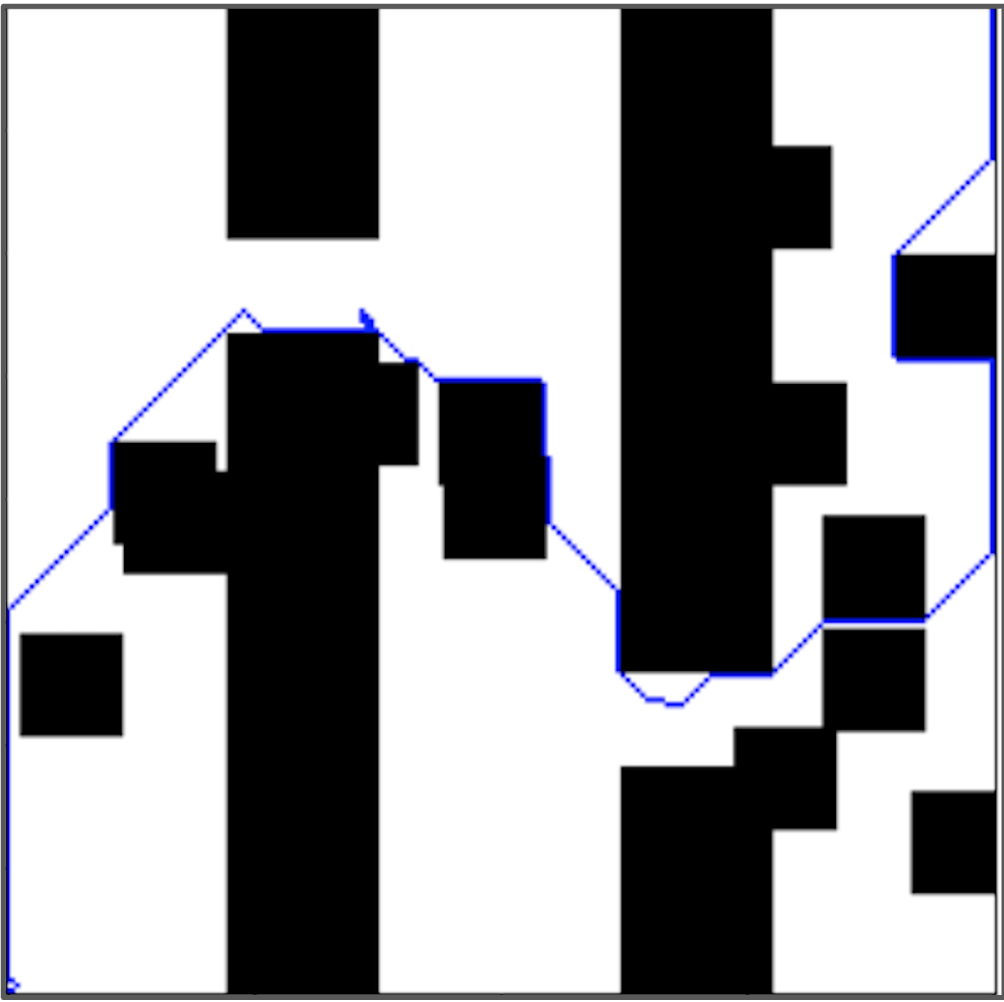
\includegraphics[width=0.49\textwidth,height=0.49\textwidth]{figures/c2.png}}%
    \caption{Gaps+Forest (\sail left, \phil right)}
    \end{subfigure}
    %%%%%%%%%%%%%%%%%%%%%%%%%%%%%%%%%%%%second row
    \begin{subfigure}[t]{0.45\textwidth}
        \raisebox{-\height}{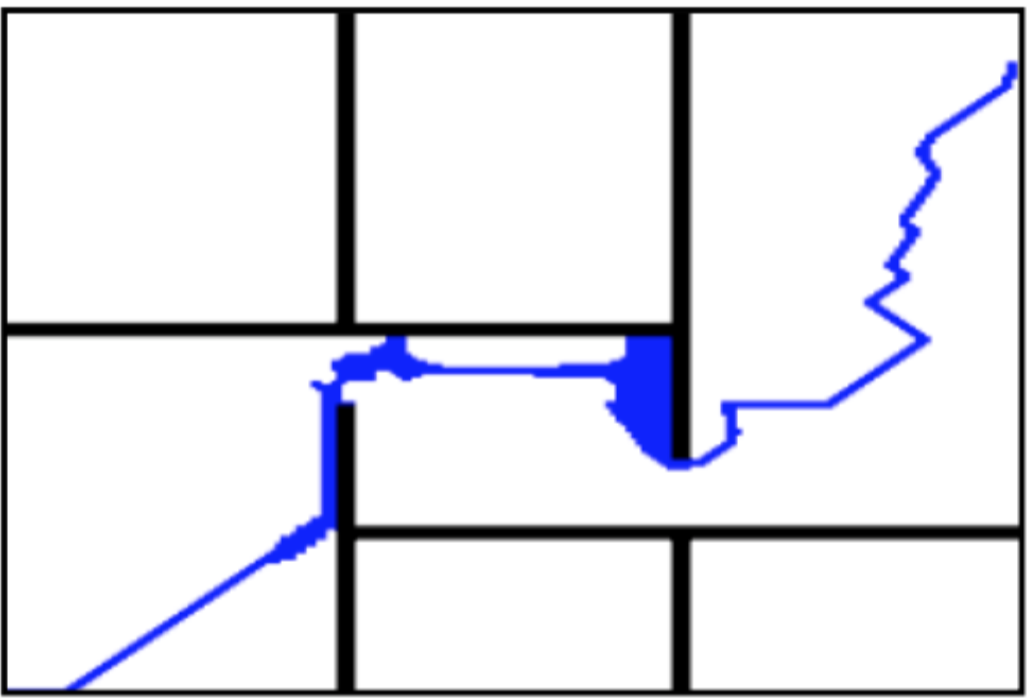
\includegraphics[width=0.49\textwidth,height=0.49\textwidth]{figures/c3_sail.png}}
        \raisebox{-\height}{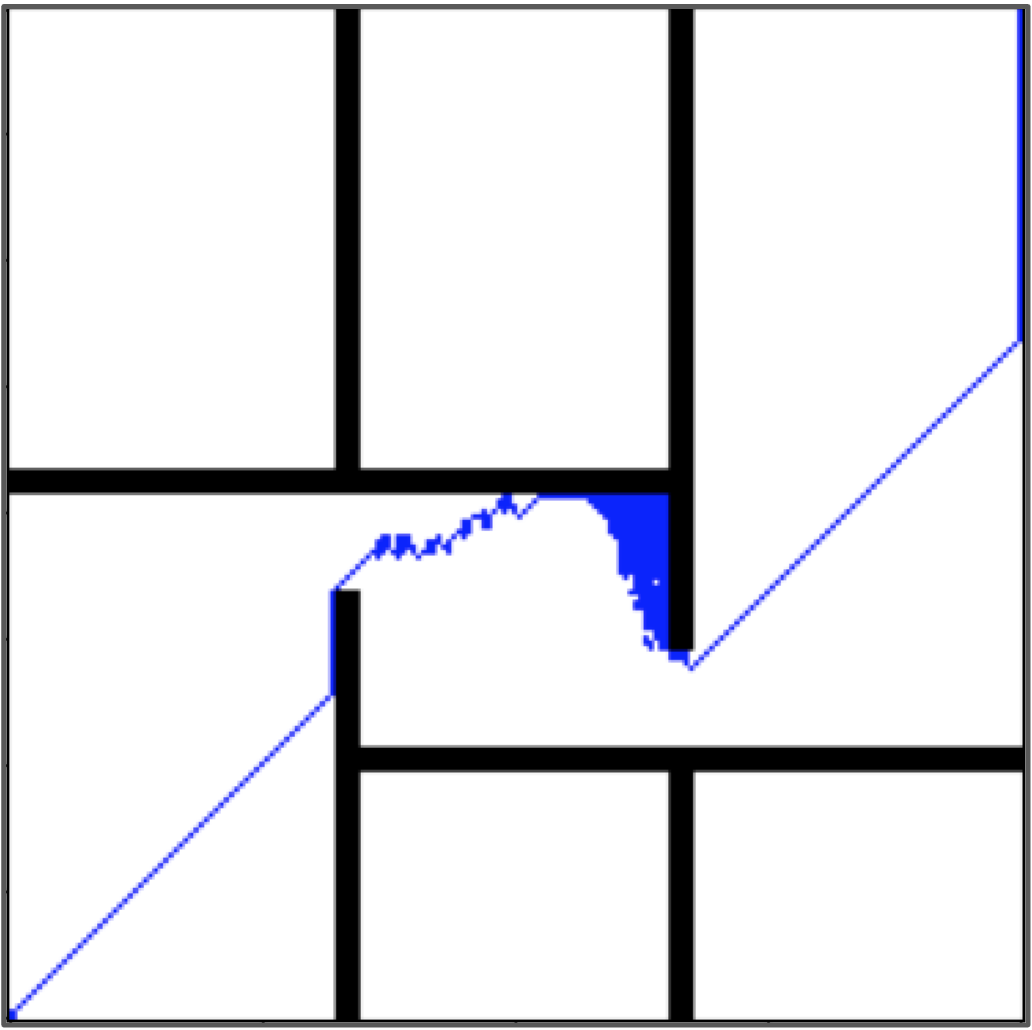
\includegraphics[width=0.49\textwidth,height=0.49\textwidth]{figures/c3.png}}%
    \caption{Mazes (\sail left, \phil right)}
    \end{subfigure}
    \hfill
    \begin{subfigure}[t]{0.45\textwidth}
          \raisebox{-\height}{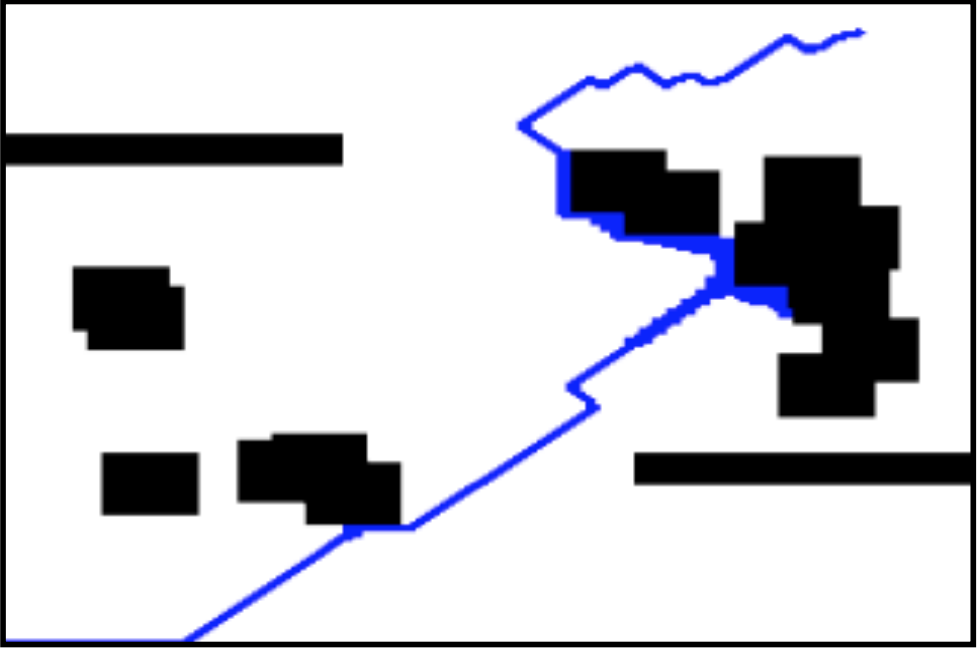
\includegraphics[width=0.49\textwidth,height=0.49\textwidth]{figures/c4_sail.png}}
          \raisebox{-\height}{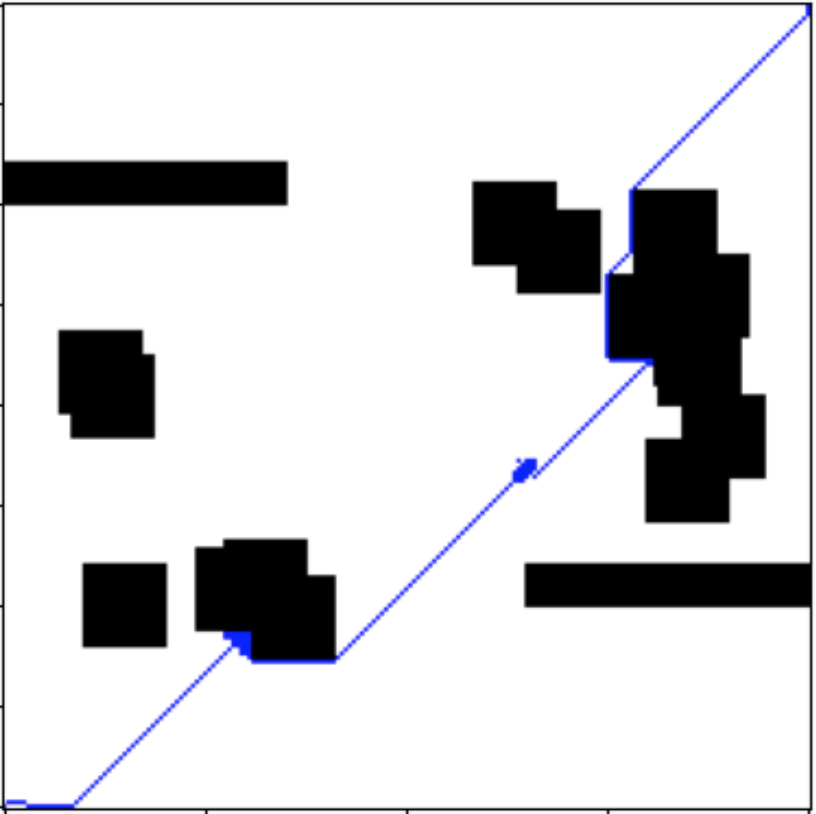
\includegraphics[width=0.49\textwidth,height=0.49\textwidth]{figures/c4.png}}%
    \caption{Forest (\sail left, \phil right)}
    \end{subfigure}
    \end{adjustbox}
    \caption{In each image pair of this figure, we provide a qualitative comparison with the \sail method. In particular, we show comparisons on the \textit{Shifting gaps}, \textit{Gaps+Forest}, \textit{Mazes}, and \textit{Forest} datasets. We can observe that \phil (right) learns the appropriate heuristics for the given dataset and makes fewer redundant expansions than \sail (left).
    %\jure{there seem to be a bug in the figure. I thought that we show the same graph but a different path.} \update{Bug should be fixed}
    } 
    \label{fig:sail-comparison}
\end{figure*}

\subsection{Search in real-life graphs of different structures}
\label{sec:experiments-diversity}

In this experiment, our goal is to demonstrate the general applicability of \phil to various graphs. We train \phil on $4$ different groups of graph datasets: citation networks, biological networks, abstract syntax trees (ASTs), and road networks. We use the same graph for citation networks and road networks for training and evaluation, and we use $100$ random $v_s, v_g$ pairs for testing. In the case of biological networks and ASTs, we usually have train/validation/test splits of $80/10/10$, and in the case of the OGB \cite{hu2020open} datasets, we use the provided splits.


\begin{table*}[!htb]
\centering
\caption{Comparison of \phil with baseline approaches on $4$ groups of datasets: citation networks, biological networks, abstract syntax trees, and road networks. "$-$" denotes being out of a 4-day's training time limit. We can observe that, on average across all datasets, \phil outperforms the best baseline per dataset by $13.4 \%$. Discounting the OGBG datasets, this number becomes $19.5 \%$.}
\label{tab:table-2}
\resizebox{\columnwidth}{!}{

\begin{tabular}{c|c|ccc|ccccccc} 
\toprule
& \textbf{Dataset} &\textbf{$|\mathcal{D}|$} &\textbf{$\bar{|\VS|}$} &\textbf{$\bar{|\mathcal{E}|}$}  & \textbf{SL} &\textbf{A*} &$h_{euc}$ &\textbf{BFS} & \textbf{\sail} & \textbf{BFWS} &\textbf{\phil} \\ \midrule
\multirow{5}{*}{Citation Networks} &Cora (Sen \etal \cite{sen2008collective}) &1 &2,708 &5,429 &2.201	&2.067	&1.000	&4.001 & 0.669 &1.378    &\textbf{0.475} \\ 
&PubMed (Sen \etal \cite{sen2008collective}))   &1 &19,717 &44,338            &2.157 &2.983	&1.000	& 3.853 & 1.196 &  1.000& \textbf{0.745}  \\ 
&CiteSeer (Sen \etal \cite{sen2008collective})) &1 &3,327 &4,732            &1.636 &1.487	&1.000	&2.190 & 1.062     &0.951  &\textbf{0.599}\\
&Coauthor (cs) (Schur \etal \cite{shchur2018pitfalls}) &1 &18,333 &81,894       &1.571	&1.069	&1.000	&2.820 & 1.941 &    1.026 &\textbf{0.835}\\
&Coauthor (physics) (Schur \etal \cite{shchur2018pitfalls}) &1 &34,493 &247,962  &4.076	&1.081	&1.000	&4.523 & $-$ & 1.012 &\textbf{0.964} \\ \midrule
\multirow{4}{*}{Biological Networks} &OGBG-Molhiv  (Hu \etal \cite{hu2020open}) &41,127 &25.5	&27.5  &1.086 &1.065 &\textbf{1.000} & 1.267 & 1.104 & 1.146 & 1.016  \\
&PPI (Zitnik \etal \cite{zitnik2017predicting})         &24 &2,372.67 &34,113.16 &0.772 &0.831 &1.000 &5.618 & 1.746 & 3.941 &\textbf{0.658}\\
&Proteins (Full) (Morris \etal \cite{morris2020tudataset})  &1,113 &39.06 &72.82 &0.995 &0.997 &1.000 &2.645 & 0.891 & 0.966 &\textbf{0.831}\\
&Enzymes (Morris \etal \cite{morris2020tudataset})            &600 &32.63 &62.14 &1.073	&1.007 &1.000 &1.358 & 1.036 & 0.992 &\textbf{0.757}\\ \midrule
\multirow{1}{*}{ASTs} &OGBG-Code2 (Hu \etal \cite{hu2020open}) &452,741 &125.2 &124.2  	&1.196  &1.013	&1.000	&1.267 & 1.029 & \textbf{0.817} & 1.219 \\ \midrule
\multirow{2}{*}{Road Networks} &OSMnx - Modena (Boeing \cite{boeing2017osmnx}) &1 &29,324 &38,309  &2.904 	&3.085	&1.000	&3.493 & 1.182 &0.997&\textbf{0.489}\\ 
&OSMnx - New York (Boeing \cite{boeing2017osmnx}) &1 &54,128 &89,618 & 39.424  &36.529	&1.000	&63.352 & 1.583&1.013 &\textbf{0.962}\\ 
\bottomrule
\end{tabular}
}
\end{table*}


%\jure{Let's add a sentence commenting on performance, let's quantify it.\\
%Also, can we add 2 more columns---size of the graph (nodes, edges).\\
%Call "city networks" "road networks".
%} \update{Added dataset stats and quantified results}

Similarly as in Section \ref{sec:experiments-grids}, our $\textsc{MLP}$ has four layers of width $128$ with \textit{LeakyReLU} activations and we use a DeeperGCN~\cite{li2020deepergcn} graph convolution with \textit{softmax} aggregation. The utilized node and edge features are the provided features in each dataset, except for a few minor modifications. We train an $\textsc{MLP}$ of depth $5$ and width $256$ using supervised learning (SL) for our learning-based baseline method. 

%Our classical baselines are greedy best-first search ($h_{euc}$) and A* with a euclidean distance heuristic on the node features and breadth-first search (BFS). In Table \ref{tab:table-2}, we report the ratio of explored nodes with respect to $h_{euc}$ after search.

\xhdr{Discussion} The results presented in Table \ref{tab:table-2} suggest that \phil can learn superior search heuristics compared with baseline methods, outperforming top baselines per dataset in terms of visited nodes during a search by $13.4 \%$ on average. Two datasets where \phil fell short compared to other baselines are the \textit{OGBG-Molhiv} and \textit{OGBG-Code2} datasets. The \textit{OGBG-Code2} dataset adopts a \textit{project split} \cite{allamanis2019adverse} and OGBG-Mohliv adopts a \textit{scaffold split} \cite{wu2018moleculenet}, both of which ensure that graphs of different structure are present in the training \& test sets. Although \phil improved upon uninformed search (BFS) in the OGB datasets, structural graph consistency is explicitly discouraged in the above-mentioned OGBG splits. Without the OGBG datasets, \phil improves on the top baselines per dataset by $19.5 \%$ on average, and upon the Euclidean node feature heuristic ($h_{euc}$) by $20.4 \%$. Note that we trained \phil up to $N = 60$ iterations, which means that it only encountered a small subset of the pathfinding problems in the single graph setting, which means that \phil had to generalize to learn useful heuristics. Even in Cora, the $|\mathcal{D}| = 1$ dataset with least number of nodes, \phil observed roughly $6,000$ node distances during training, which is less than $0.2 \%$ of total distances in the Cora graph.

%The \textit{OGBG-Molhiv} and \textit{OGBG-Code2} datasets contain a diverse set of molecules (approx. $40, 000$) and code-bases (approx. $400, 000$), respectively. Contrary to the grid datasets from our previous experiments, where both train and test datasets were structurally similar




%\jure{Same here, can we quantify performance: PHIL explores X\% less nodes on average than the second best method.} \update{Should be better quantified}


%\jure{This is interesting but perhaps not too important. We can cut it and use space to make the method description less dense} \xhdr{Road network results} Further, we can observe the difference in the performance of \phil on the \textit{OSMnx - Modena} and \textit{OSMnx - New York} \cite{boeing2017osmnx} networks. The network of New York resembles a regular grid-like graph, where using naive heuristics is close to optimal. On the other hand, Modena presents a more irregular graph structure, where purely distance minimizing expansions are often incorrect. The relative irregularity of Modena is also evidenced by the fact that in the graph of New York, distance minimizing expansions yield on average $|\VS_{seen}|$ only $6\times$ larger than the lengths of shortest paths, while in Modena, this number is approximately $60$. \phil can bring significant upsides to the euclidean heuristic, especially when the euclidean heuristic is far from optimal. We can conclude that the main use-cases of \phil are in applications where the graphs present in the application domain are structurally similar to training datasets, and where feature distance minimizing expansions are not close to optimal.

\subsection{Planning for drone flight}
\label{sec:experiments-drone}

%Suppose that we wish to operate an autonomous UAV in a densely populated indoor area. An essential component of our UAV would be a planning module, which is classically implemented by treating the environment as a dense 3D grid graph and running a pathfinding algorithm such as A*. In practice, due to our UAV's limited onboard computation capabilities \cite{liu2018motion}, node expansion becomes a performance bottleneck, especially as it can include a complex set of collision and regulation compliance checks. We may relax the shortest path requirement and include additional heuristics in our search algorithm to solve this issue. However, coming up with heuristics that minimize search effort is not a trivial task, as these can depend on the structure of the environment, the local regulations, and possibly the geometry of the UAV.


\begin{wrapfigure}[17]{r}{0.4\textwidth}
  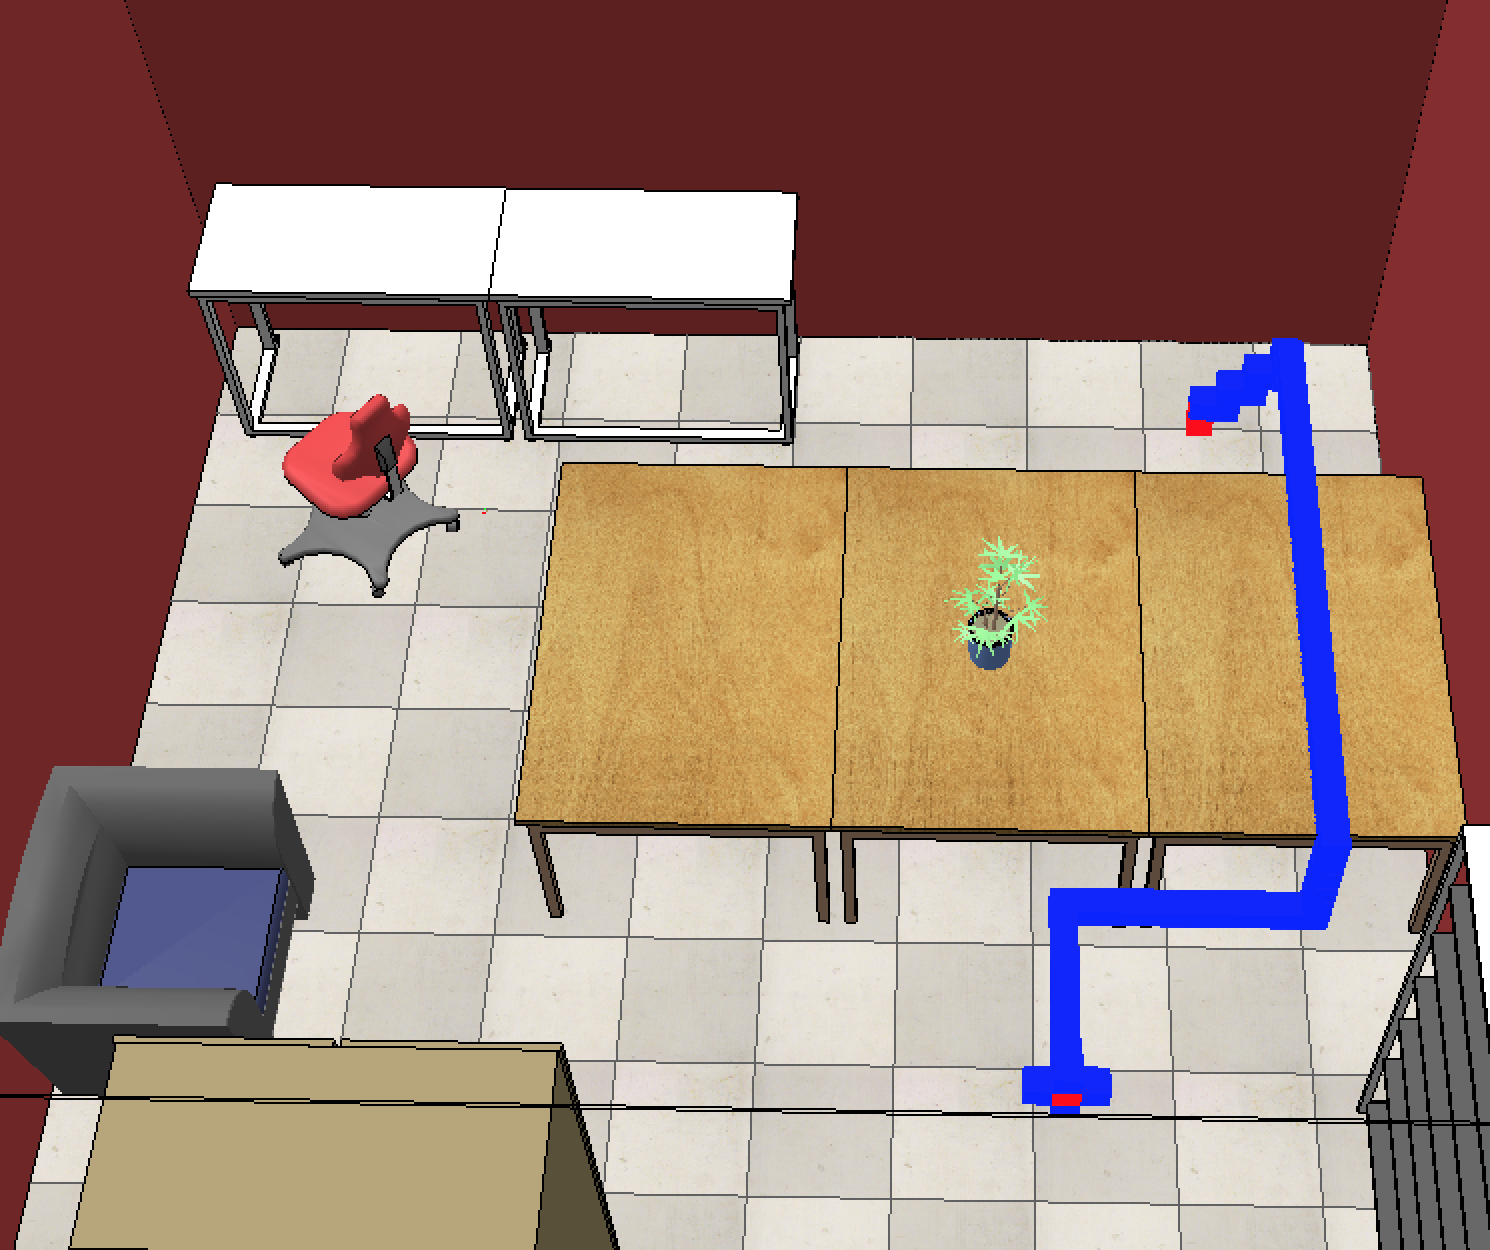
\includegraphics[width=0.9\linewidth]{figures/planned_path.png}
    \caption{This figure illustrates the \textit{room adversarial} environment with an example planning problem (red) and the expanded graph by \phil (blue).}
  \label{fig:room-adv}
\end{wrapfigure}

In our final experiment, we use \phil to plan collision-free paths in a practical drone flight use case within an indoor environment. We built our environment using the CoppeliaSim simulator \cite{coppeliaSim}, and the Ivy framework \cite{lenton2021ivy}. Figure \ref{fig:room-adv}  presents the environment which we refer to as \textit{room adversarial} in Table \ref{tab:table-3}. We discretize the environments into 3D grid graphs of size $50 \times 50 \times 25$, and randomly remove $5$ sub-graphs of size  $5 \times 5 \times 5$ both during training and testing, this way simulating real-life planning scenarios with random obstacles. The hyperparameter configuration and the specific architecture we utilize are equivalent to Section \ref{sec:experiments-grids}, but with $n = 4$. Likewise, the node features are 3D grid coordinates, and the baselines include supervised learning (SL), $h_{euc}$, A*, and BFS, similarly as in Sections \ref{sec:experiments-grids}, \ref{sec:experiments-diversity}. In Table \ref{tab:table-3} we report the ratio of expanded nodes with respect to $h_{euc}$. 

\xhdr{Video demo} We provide a video demonstration of \phil running in \textit{room adversarial}: \url{https://cutt.ly/eniu5ax}.
\begin{table*}[!htb]
\centering
\caption{Results of \phil in the context of planning for indoor UAV flight. \phil outperforms all baselines in both the \textit{room simple} and \textit{room adversarial} environments while remaining close performance-wise to the optimal number of expansions.}
\label{tab:table-3}
\resizebox{0.7\columnwidth}{!}{%

\begin{tabular}{cccccccc|c} \toprule
 \textbf{Dataset}                     & \textbf{SL} &\textbf{A*} & $h_{euc}$ & \textbf{BFS} & \textbf{\sail} & \textbf{BFWS} & \textbf{\phil} & \textbf{Shortest path} \\ \midrule
Room simple   & 1.124 & 76.052  & 1.000 & 291.888 & 0.973 & 1.286 & \textbf{0.785} &0.782                 \\ 
Room adversarial  & 2.022 & 67.215   & 1.000 & 238.768 & 0.944 & 1.583 & \textbf{0.895} & 0.853                  \\ \bottomrule
\end{tabular}
}
\end{table*}

\xhdr{Discussion} As we can observe in Table \ref{tab:table-3}, \phil outperforms all baselines in both environments. Interestingly, \phil expands only approximately $0.3\%$ more nodes in the simple room than least possible and $4.9\%$ more in the adversarial room case. The same figures for the greedy method ($h_{euc}$) are $27.8\%$  and $17.2 \%$, respectively. These results indicate that \phil is capable of learning planning strategies that are close to optimal in both \textit{simple} and \textit{adversarial} graphs, while the performance of naive heuristics degrades.

\subsection{Runtime Analysis}
\label{sec:runtime}
We evaluated the inference runtimes of seven approaches on all datasets in Section~\ref{sec:experiments-grids}. Each approach's runtime was normalized by the number of nodes it visited. The runtime experiments were conducted on a machine with an RTX5000 GPU and an Intel Xeon 5222 CPU.

\begin{figure}[H]
    \centering
    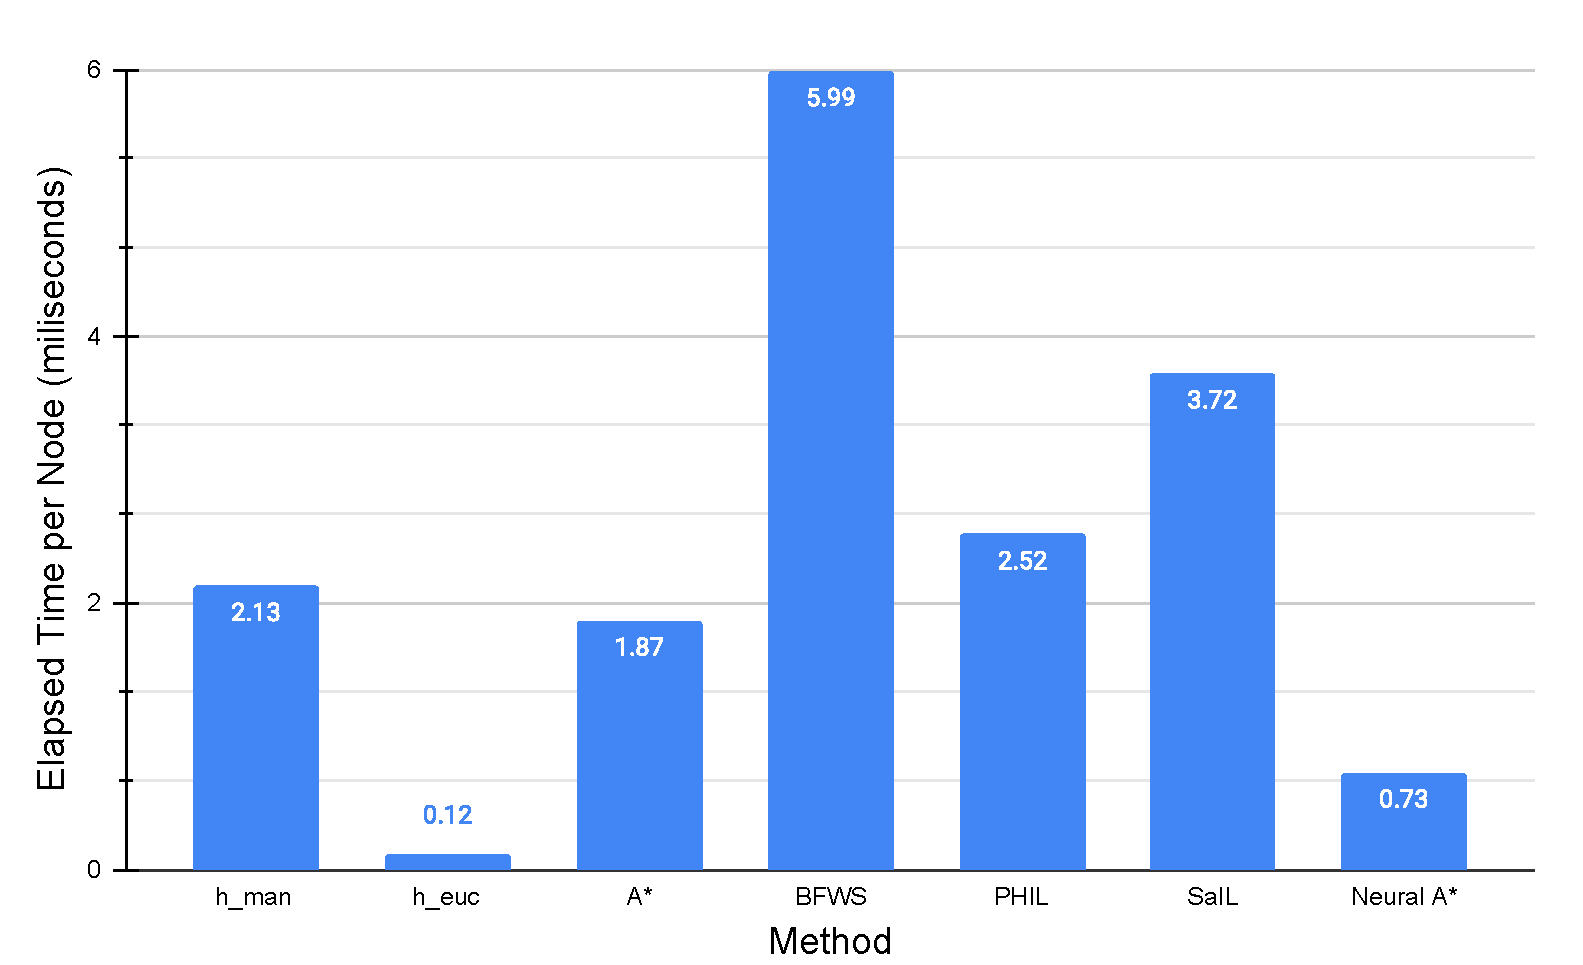
\includegraphics[width=0.9\linewidth]{PHIL/figures/runtime.pdf}
    \caption{Timing experiments on grid search datasets \cite{bhardwaj2017learning}.}
    \label{fig:phil-runtime}
\end{figure}

Figure~\ref{fig:phil-runtime} summarizes the test runtimes of the different approaches. PHIL runs $57.9\%$ faster than BFWS and $32.2\%$ faster than \sail , and not much slower than traditional A* ($34.7\%$) and $h_{man}$ ($18.3\%$). Although Neural A* is $71.0\%$ faster than PHIL due to the fact that it casts the whole search process into matrix operations on images, it cannot be employed in a generic search setting.